\section{Durchführung}
\label{sec:Durchführung}
Zunächst werde eine Kennlinienschar erstellt indem in geeigneten Intervallen dem Aufbau die Beschleunigungspannung $U_B$ sowie der Saugstrom $I_\text{S}$ entnommen wird. Dies wird für 5 verschiedene Heizströme wiederholt. Bei der Berechnung der Spannungen und Ströme sind die einzelnen Widerstände die die einzelnen Bauteile besitzen zu beachten. Desweiteren soll der Heizstrom wie auch die Spannung notiert werden.

Zur Messung des Anlaufstromkurve ist der Aufbau wie in Abbildung \ref{fig:Anl} zu tätigen.
\begin{figure}
  \centering
  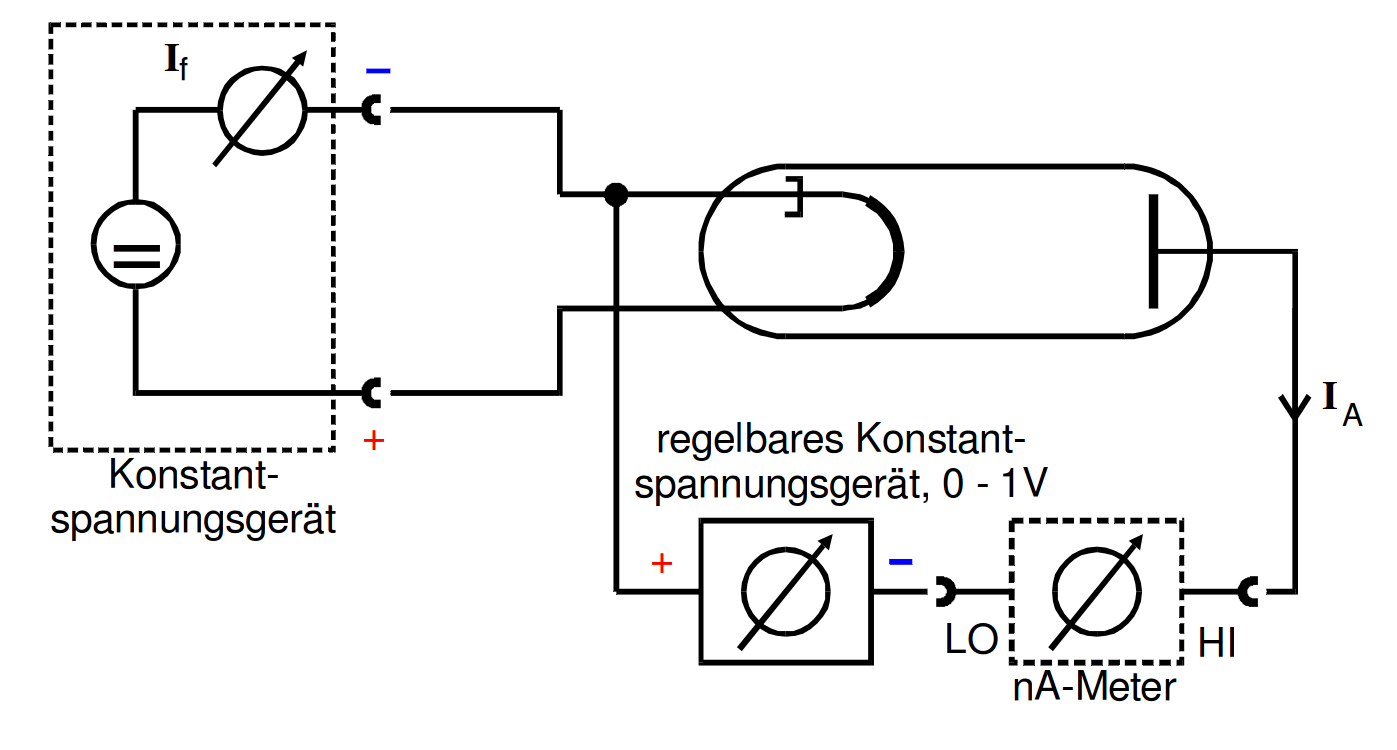
\includegraphics[height=5cm]{picture/Gegenfeld.png}
  \caption{Anlaufsstromschaltung \cite{pra}}
  \label{fig:Anl}
\end{figure}
Dabei wird in 20 äquidistanten Schritten zwischen, 0 und 1 Volt ein Gegenfeld aufgebaut. Der Heizstrom ist zu Maximieren und die Ströme im nA Bereich vom Messgerät abzulesen. Dabei ist der Widerstand des Bananensteckers durch mehrfaches drehen zu minimieren.
\newpage
